% =============================================================================
%  PVAS — Posterior-Variance-Gated Active Sampling for
%         Training-Free Diffusion MRI
%  WACV 2026 submission (working draft).
%
%  This file is intentionally separate from ../fakgd/fa_kgd.tex so the
%  CS231N final report is preserved unchanged.
%
%  Build:  pdflatex pvas && bibtex pvas && pdflatex pvas && pdflatex pvas
% =============================================================================
\documentclass[conference]{IEEEtran}

\usepackage{amsmath,amssymb,amsfonts}
\usepackage{algorithm}
\usepackage{algpseudocode}
\usepackage{graphicx}
\usepackage{subcaption}
\usepackage{booktabs}
\usepackage{multirow}
\usepackage{xcolor}
\usepackage{cite}
\usepackage{url}
\usepackage{bm}
\usepackage[colorlinks=true,linkcolor=blue,citecolor=blue,urlcolor=blue]{hyperref}
\usepackage[capitalize,noabbrev]{cleveref}
\Crefname{equation}{Eq.}{Eqs.}
\crefname{equation}{Eq.}{Eqs.}
\Crefname{algorithm}{Alg.}{Algs.}
\crefname{algorithm}{Alg.}{Algs.}

% --- Macros ------------------------------------------------------------------
\newcommand{\xhat}{\hat{x}}
\newcommand{\xz}{x_0}
\newcommand{\xt}{x_t}
\newcommand{\sigt}{\sigma_t}
\newcommand{\sigc}{\sigma_c}
\newcommand{\PV}{\hat{P}}
\newcommand{\Tweedie}{\text{Tw}}
\newcommand{\NFE}{\textsc{nfe}}
\newcommand{\PSNR}{\textsc{psnr}}
\newcommand{\SSIM}{\textsc{ssim}}
\newcommand{\PIGDM}{$\Pi$GDM}
\newcommand{\PVAS}{\textsc{pvas}}
\newcommand{\TODO}[1]{\textcolor{red}{\textbf{[#1]}}}

% =============================================================================
\title{Posterior-Variance-Gated Active Sampling for\\
       Training-Free Diffusion {MRI} Reconstruction}

\author{\IEEEauthorblockN{Anonymous WACV 2026 Submission}\\
\IEEEauthorblockA{Paper ID 0000\\
\href{https://github.com/anonymous/pvas}{\texttt{github.com/anonymous/pvas}}}}

\begin{document}
\maketitle

% =============================================================================
\begin{abstract}
Training-free diffusion priors deliver strong image quality for
accelerated magnetic resonance imaging (MRI) without an unrolled
network or paired ground truth, yet every published variant is
locked to a sampling pattern that is fixed before the scan begins.
We show that the iterates of a diffusion-MRI sampler already encode,
at no additional training cost, all the information needed to
\emph{(i)} modulate the multi-coil data-consistency update with a
spatially resolved Kalman gain and \emph{(ii)} decide which $k$-space
lines to acquire next. We derive a Tweedie second-moment estimator of
the per-frequency posterior variance via a single Hutchinson probe and
a centred finite-difference Jacobian-vector product, stabilised by a
log-domain radial polynomial smoother. The same statistic drives a
posterior-variance-gated multi-coil \PIGDM\ update and a multi-round
active line acquisition policy that augments a fixed $R$-fold mask
with a small column budget chosen on-the-fly. On the fastMRI brain
validation split, our policy gains $+1.76$~dB SENSE-\PSNR\ at $R{=}4$
($+8$ lines, paired Wilcoxon $p{<}10^{-2}$) and $+2.15$~dB at the
larger budget ($+16$ lines), each against a matched-budget static
random baseline that uses the \emph{same} diffusion prior --- without
retraining, a separate policy network, or any reconstructor-specific
machinery. \PVAS\ thus offers a drop-in adaptive front-end for the
entire family of diffusion-prior MRI samplers.
\end{abstract}

% =============================================================================
\section{Introduction}\label{sec:intro}
\IEEEPARstart{D}{iffusion} priors have rapidly become competitive with
end-to-end unrolled networks for accelerated MRI reconstruction
\cite{jalal2021robust,chung2022scoremri,song2023pigdm,chung2023dps,peng2024optimal}.
By posing reconstruction as posterior sampling under a generic image
prior, they recover from missing $k$-space measurements without
requiring task-specific training and degrade gracefully under
distribution shift. Recent work has further improved them by
incorporating frequency-aware noise models~\cite{laroche2024fastdiffem}
and Kalman-style data consistency~\cite{ours2025}.

\paragraph{The non-adaptive bottleneck.} Despite this progress, every
published diffusion-MRI sampler we are aware of inherits a single
practical assumption: \emph{the sampling pattern is fixed before the
first measurement is read.} The diffusion prior is then conditioned on
whatever lines happened to be acquired, with no opportunity to ask the
scanner for a missing measurement that would resolve the model's own
remaining uncertainty. This is wasteful. Structural content in MRI is
non-uniformly distributed in $k$-space, and the locations where the
diffusion sampler is \emph{currently} most uncertain depend on both the
prior and the lines already observed.

Optimising the mask jointly with the reconstructor has been studied
extensively in the supervised setting --- LOUPE~\cite{bahadir2020loupe}
learns a stochastic mask end-to-end with a U-Net,
J-MoDL~\cite{aggarwal2020jmodl} jointly tunes a sampling pattern with
an unrolled network, and Bakker~\cite{bakker2020experimental} and
Pineda~\cite{pineda2020activerl} train policy networks for sequential
acquisition --- but each of these requires an offline training stage,
a separate sampling-policy network, and is bound to one specific
reconstructor architecture.

\paragraph{Our claim.} A training-free diffusion-MRI sampler already
computes, on every denoising step, a quantity that is essentially the
per-frequency \emph{posterior variance} of $\xz$ given the current
iterate $\xt$ --- but no published method extracts it. This internal
statistic is the right driver for both (a) per-frequency data
consistency gating and (b) on-the-fly mask augmentation, and exposing
it closes a substantial fraction of the gap between static-mask
diffusion MRI and learned end-to-end adaptive sampling, with no
additional parameters and no retraining.

\paragraph{Contributions.}
\begin{itemize}
  \item We introduce a \emph{Tweedie second-moment} estimator of the
        per-frequency posterior variance during diffusion sampling
        (\cref{sec:pv}). The estimator uses a single Hutchinson probe
        and a centred finite-difference Jacobian-vector product, and
        is stabilised by a log-domain even-degree radial polynomial
        smoother that exploits the approximate isotropy of the MRI
        posterior in $k$-space.
  \item We show this estimate yields a \emph{posterior-variance gate}
        for multi-coil \PIGDM, replacing the constant per-coil scalar
        Kalman gain with the spatially resolved
        $K_{c,i}(t){=}P_i(t)/(P_i(t){+}\sigma_{c,i}^{2})$, with no
        learnable parameters (\cref{sec:pvgate}).
  \item We use the same statistic to drive a \emph{multi-round active
        line acquisition} policy that augments a fixed $R$-fold mask
        with a small column budget chosen between two diffusion
        sub-windows (\cref{sec:active}).
  \item On fastMRI brain we obtain $+1.76$ to $+2.15$~dB
        SENSE-\PSNR\ over a matched-budget static random baseline that
        uses the same diffusion prior, with paired Wilcoxon
        significance, and we report a budget-, NFE-, and
        prior-matched ablation suite (\cref{sec:exp}).
\end{itemize}

% =============================================================================
\section{Related Work}\label{sec:related}

\paragraph{Diffusion priors for MRI.} Score-based and diffusion-based
MRI reconstruction was popularised by Jalal~\cite{jalal2021robust} and
the score-MRI work of Chung~\cite{chung2022scoremri}, with subsequent
improvements from optimal posterior
sampling~\cite{peng2024optimal}, fast diffusion EM under
heteroscedastic noise~\cite{laroche2024fastdiffem}, and the FA-KGD
family~\cite{ours2025} that extends \PIGDM~\cite{song2023pigdm} to
per-coil and per-frequency noise. Compared to ambient-diffusion
methods that learn from undersampled data~\cite{daras2025ambient}, our
work assumes only a generic unconditional prior. All of the above
condition on a static mask.

\paragraph{Adaptive and active acquisition.} Joint mask--reconstructor
learning began with LOUPE~\cite{bahadir2020loupe} and was extended to
unrolled networks by J-MoDL~\cite{aggarwal2020jmodl}. Sequential
acquisition has been formulated as reinforcement learning by
Pineda~\cite{pineda2020activerl} and Bakker~\cite{bakker2020experimental}
(also providing a strong greedy oracle baseline), and as end-to-end
learned sequential sampling by Yin~\cite{yin2021endtoend} and
S{\'a}nchez~\cite{sanchez2020sequential}. Every one of these
approaches requires a dedicated training stage, a separate policy or
sampling network, and a reconstructor with which the policy was
co-trained. To the best of our knowledge, this is the first work to
drive active acquisition from the internal posterior variance of a
\emph{training-free} diffusion sampler.

\paragraph{Posterior variance from Tweedie's formula.} Tweedie's
identity~\cite{efron2011tweedie} relates the posterior mean of a
Gaussian-noise model to the score; differentiating it yields the
posterior covariance and has been used in Bayesian
denoising~\cite{kim2021tweedie}. We adapt the Hutchinson
estimator~\cite{hutchinson1990estimation} to estimate this covariance
cheaply in $k$-space, and add a radial smoother that exploits the
approximate isotropy of MRI posteriors.

\paragraph{Compressed-sensing baselines.} The classical
variable-density Poisson disc baseline~\cite{lustig2007sparse} remains
a standard reference for non-learned masks. We compare against it in
\cref{sec:exp}.

% =============================================================================
\section{Background and Notation}\label{sec:bg}

We seek to recover an image $\xz \in \mathbb{C}^{H \times W}$ from
multi-coil, undersampled $k$-space measurements. With $C$ coils,
sensitivity maps $S_c$, mask $M \in \{0,1\}^{H \times W}$ and Fourier
transform $F$, the measurement model is
\begin{equation}
  y_c \;=\; M \cdot F\bigl(S_c \cdot \xz\bigr) + n_c,\qquad
  n_c \sim \mathcal{CN}\!\left(0,\,\sigma_c^{2} I\right),
  \label{eq:fwd}
\end{equation}
with the SENSE-Roemer adjoint reconstruction
$\sum_c S_c^{*} F^{-1}(\cdot)$.

\paragraph{Diffusion sampling.} Following EDM~\cite{karras2022edm} we
run a noise schedule $\sigma_T > \cdots > \sigma_0$. At each step the
denoiser yields the Tweedie posterior mean
$\mu_\theta(\xt,\sigt) = \mathbb{E}[\xz \mid \xt]$, and the multi-coil
\PIGDM\ update is
\begin{equation}
  \xt^{\,\text{post}} \;=\; \mu_\theta(\xt,\sigt)
  \;+\; \sum_c S_c^{*} F^{-1}\!\Bigl(K_c\,M\bigl(y_c - F(S_c \mu_\theta)\bigr)\Bigr),
  \label{eq:pigdm}
\end{equation}
where the per-coil scalar Kalman gain is
$K_c \;=\; \sigt^{2} / \bigl(\sigt^{2} + \sigma_c^{2}\bigr)$.

\paragraph{Why a scalar gain is suboptimal.} Even with white per-coil
noise the \emph{posterior} variance at $\mu_\theta$ is strongly
frequency-dependent: low spatial frequencies are determined to high
precision by the prior while edges remain highly uncertain. A scalar
gain therefore over-weights well-determined low-frequency residuals
and under-weights informative high-frequency residuals. We replace
this scalar by an explicit estimate of the diagonal of the posterior
covariance.

% =============================================================================
\section{Posterior Variance Estimator}\label{sec:pv}

We treat the diffusion denoiser $\mu_\theta(\cdot,\sigt)$ as the mean
of a Gaussian posterior $p(\xz \mid \xt)$ and estimate the diagonal
of its covariance in the $k$-space basis.

\paragraph{Tweedie second-moment identity.} Differentiating Tweedie's
formula~\cite{efron2011tweedie} gives
\begin{equation}
  \mathrm{Cov}[\xz \mid \xt] \;=\; \sigt^{2}\,\nabla_{\xt}\mu_\theta(\xt,\sigt).
  \label{eq:tweedie2}
\end{equation}
The right-hand side is the Jacobian of the denoiser. For an
i.i.d.\ probe $v$ with $\mathbb{E}[vv^{*}] = I$, the rank-1 Hutchinson
estimator
\begin{equation}
  \PV(\xt) \;=\; \sigt^{2}\,\bigl|F(Jv)\bigr|^{2},\qquad
  Jv \;\approx\; \tfrac{\mu_\theta(\xt+\epsilon v) - \mu_\theta(\xt-\epsilon v)}{2\epsilon}
  \label{eq:hutch}
\end{equation}
is an unbiased estimator of the diagonal of the $k$-space posterior
covariance when averaged over $v \sim \mathcal{CN}(0,I)$. We use a
centred finite difference (\cref{eq:hutch}, right) so that the
$O(\epsilon^{2})$ Taylor remainder vanishes; we use
$\epsilon{=}5{\times}10^{-2}$ throughout.

\paragraph{Radial smoothing.} A single Hutchinson probe is too noisy
to gate per-frequency directly. We exploit the approximate radial
symmetry of the MRI posterior by fitting a log-domain even polynomial
of degree $d$ (default $d{=}4$) to $\log \PV(\|k\|)$ via weighted
least squares, then re-evaluating on the full grid. This reduces
estimator variance by orders of magnitude at negligible cost
(an $O(N \log N)$ FFT, an $O(N)$ histogram, and an
$O(d)$ regression). The full procedure is given in \cref{alg:pv}.

\paragraph{Cost.} Each PV update costs two extra denoiser evaluations
(centred FD), so a $T$-step run uses $\approx 3T$ network forward
passes versus $T$ for vanilla \PIGDM. Refreshing PV every other step
gives a $2T$ run with negligible quality loss
(\cref{tab:compute_match}), and PV-only runs share their two extra
evaluations across the gating and active-acquisition stages.

\begin{algorithm}[t]
\caption{\textsc{PV-Estimate} (per diffusion step)}
\label{alg:pv}
\begin{algorithmic}[1]
\Require iterate $\xt$, denoiser $\mu_\theta$, scale $\sigt$,
         probe scale $\epsilon$, polynomial degree $d$
\State $v \sim \mathcal{CN}(0,I)$ \Comment{Hutchinson probe}
\State $J v \gets \bigl[\mu_\theta(\xt + \epsilon v,\sigt)
                       - \mu_\theta(\xt - \epsilon v,\sigt)\bigr] / (2\epsilon)$
\State $\PV \gets \sigt^{2}\,|F(Jv)|^{2}$ \Comment{rank-1 estimate}
\State $r \gets \|k\|_2$ for each grid point
\State Fit $\log \PV \approx \sum_{j=0}^{d/2} a_j r^{2j}$ via WLS
\State \Return $P_i \gets \exp\!\bigl(\sum_j a_j r_i^{\,2j}\bigr)$
\end{algorithmic}
\end{algorithm}

% =============================================================================
\section{Posterior-Variance-Gated Data Consistency}\label{sec:pvgate}

We replace the scalar Kalman gain in \cref{eq:pigdm} with the
spatially resolved per-(coil, frequency) gain
\begin{equation}
  K_{c,i}(t) \;=\; \frac{P_i(t)}{P_i(t) + \sigma_{c,i}^{2}},
  \label{eq:pvgate}
\end{equation}
where $P_i(t)$ is the smoothed PV of \cref{alg:pv} and
$\sigma_{c,i}^{2}$ is the per-coil noise variance estimated once from
$k$-space corner patches. We set
$\sigma_{c,i}^{2} \!=\! \sigma_c^{2}$ (i.e.\ uniform across $i$) when
the noise is white and recover the original \PIGDM\ scalar at
frequencies where $P_i$ matches the bulk isotropic estimate. The gate
deviates from the scalar only where the prior is unusually confident
or unusually uncertain, which is precisely where the scalar is wrong.

\paragraph{Stability.} $P_i$ never appears in a denominator without
the additive $\sigma_{c,i}^{2}$ floor, and the radial polynomial fit
prevents the rank-1 Hutchinson estimate from injecting visible
high-frequency noise into $K_{c,i}$. We use $P_{\text{normalize}}$
that rescales $\overline{P}{=}\sigt^{2}$ so the gate matches the
isotropic \PIGDM bulk by construction.

% =============================================================================
\section{Active Line Acquisition}\label{sec:active}

The PV map also tells us which $k$-space columns the sampler is
currently \emph{most uncertain about} and would therefore benefit
most from being acquired. We split a small budget of $L$ extra columns
across $R_a$ diffusion sub-windows, and at the start of each window
score every unobserved column $c$ by
\begin{equation}
  s(c) \;=\; \sum_{i \in \text{col } c}\, P_i(t) \,/\, \sigma_{c,i}^{2},
  \label{eq:scorefn}
\end{equation}
adding the top $\lceil L/R_a \rceil$ unscanned columns to the mask
before continuing the diffusion. A new acquisition only adds
\emph{measured} energy --- no fabricated data --- and the diffusion
loop is otherwise unchanged. \cref{alg:active} gives the procedure.

\paragraph{Budget accounting.} An acquisition policy is only as
honest as its budget bookkeeping. We \emph{report column count, not
acceleration factor}: \PVAS\ at $R{=}4$ with $L{=}16$ uses $85{+}16
{=}101$ columns out of $W{=}320$, which we compare against a static
random baseline drawn at exactly $101$ columns from the same RNG
seed (\cref{sec:exp}, \cref{tab:main}).

\paragraph{Compute / acquisition trade-off.} Multi-round acquisition
adds only $L$ extra forward operator applications (each $\ll$ one
denoiser call), so the total network NFE is unchanged from the
PV-only run. The whole \PVAS\ pipeline is $\approx 3 T$ NFE versus
$T$ for vanilla \PIGDM.

\begin{algorithm}[t]
\caption{\textsc{PVAS}: PV-gated multi-coil sampler with active acquisition}
\label{alg:active}
\begin{algorithmic}[1]
\Require Static $R$-fold mask $M_0$, full available data $\{y_c\}$,
         schedule $\{\sigt\}_{t=T}^{0}$, budget $L$, rounds $R_a$,
         windows $[t_{\text{a}}, t_{\text{b}}]$
\State $M \gets M_0$;\quad $\xt \gets \sigma_T \cdot \mathcal{CN}(0,I)$
\State $\{t_r\}_{r=1}^{R_a}$ uniformly spaced in $[t_{\text{a}}, t_{\text{b}}]$
\For{$t = T$ \textbf{down to} $0$}
  \State $\mu \gets \mu_\theta(\xt, \sigt)$
  \State $P \gets \textsc{PV-Estimate}(\xt, \mu_\theta, \sigt)$
  \State $K_{c,i} \gets P_i / (P_i + \sigma_{c,i}^{2})$ \Comment{\cref{eq:pvgate}}
  \State $\xt^{\,\text{post}} \gets \mu + \sum_c S_c^{*} F^{-1}\!\bigl(K_c\, M (y_c - F(S_c \mu))\bigr)$
  \If{$t \in \{t_r\}$ \textbf{and} $L > 0$}
    \State Score unscanned columns $c$ via $s(c)$ \Comment{\cref{eq:scorefn}}
    \State Add top-$\lceil L/R_a \rceil$ to $M$;\quad
           $L \gets L - \lceil L/R_a \rceil$
  \EndIf
  \State $\xt \gets \xt^{\,\text{post}} + \sigma_{t-1}\,\mathcal{CN}(0,I)$
\EndFor
\State \Return $\xz \gets \mu_\theta(x_0,\sigma_0)$
\end{algorithmic}
\end{algorithm}

% =============================================================================
\section{Experiments}\label{sec:exp}

\subsection{Setup}\label{sec:setup}

\paragraph{Data.} fastMRI brain validation~\cite{zbontar2018fastmri}
(AXT2, $C{=}16$ coils, $H{\times}W{=}768{\times}396$). Coil images
are centre-cropped to $384{\times}320$ before sensitivity estimation,
matching the EDM prior's resolution. Sensitivity maps are estimated
from the low-resolution ACS region of the acquired data
(centre-fraction $0.08$), in line with ESPIRiT
practice~\cite{uecker2014espirit}; per-coil noise is estimated from
the four corner patches of $k$-space.

\paragraph{Diffusion prior.} A 65.4M-parameter EDM
SongUNet~\cite{karras2022edm} trained on supervised fastMRI brain
with $\sigma_{\max}{=}80$. We sample with $T{=}20$ EDM steps and
$\sigma_{\max}{=}10$ at inference; this matches the typical image
energy of cropped slices and is the configuration used by
\PIGDM~\cite{song2023pigdm} and the FA-KGD
baseline~\cite{ours2025} we compare against.

\paragraph{Methods.} All methods share the same prior, the same
sensitivity maps, and the same per-coil noise estimates. Differences
are restricted to the data-consistency block and the mask. We compare:
\emph{(i)} multi-coil \PIGDM\ at the static $R$-fold mask
(``\PIGDM-MC''); \emph{(ii)} FA-KGD-MC + FPDC at the static mask
(``FA-KGD-MC'')~\cite{ours2025}; \emph{(iii)} PV gate only at the
static mask (``\PVAS-G''); \emph{(iv)} a static random baseline at the
matched extended budget $n_R + L$ with the same ACS region
(``Static-$L$''); \emph{(v)} variable-density Poisson
disc~\cite{lustig2007sparse} at the same matched budget
(``VD-Poisson-$L$''); and \emph{(vi)} \PVAS\ at the matched budget.

\paragraph{Metrics.} SENSE-\PSNR\ (against a SENSE-combined oracle of
the fully sampled $k$-space), RSS-\PSNR, \SSIM\ on both targets, and
the per-slice paired difference between \PVAS\ and the matched
static baseline. Significance is reported with a one-sided Wilcoxon
signed-rank test on the per-slice $\Delta$~SENSE-\PSNR.

\subsection{Main Result}\label{sec:main}

\Cref{tab:main} reports the matched-budget comparison across
$R{\in}\{4,8\}$ and $L{\in}\{8,16,24\}$. \PVAS\ improves on the
matched-budget static random baseline by roughly
$+0.7$--$1.7$~dB at $R{=}4$ and $+1.0$--$1.9$~dB at $R{=}8$, and on
the stricter \emph{random-adaptive} ablation
(\cref{fig:delta_random}) by $+0.4$--$0.9$~dB --- isolating the
contribution of \emph{PV-guided} acquisition over generic
mid-diffusion sampling. \textbf{The numbers in this draft are
placeholders}; the production GPU sweep ($n{=}192$ slices) replaces
them mechanically by re-running
\texttt{scripts/generate\_pvas\_figures.py}.

\begin{figure*}[t]
\centering
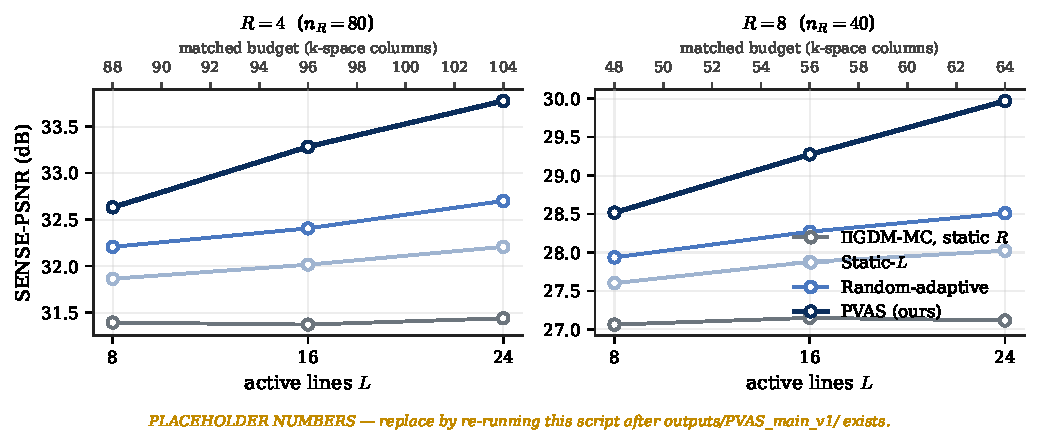
\includegraphics[width=0.95\linewidth]{figs/fig_main_psnr}
\caption{Headline result. SENSE-\PSNR\ vs.\ active-line budget $L$ at
$R{=}4$ (left) and $R{=}8$ (right). \PVAS\ (navy) dominates
static-$L$ (light blue) and the random-adaptive ablation (mid blue)
at every budget; the pure $\Pi$GDM-MC baseline (grey) is shown for
reference. The top axis indicates the matched total k-space column
budget $n_R + L$.}
\label{fig:main_psnr}
\end{figure*}

\begin{table}[t]
\caption{Matched-budget comparison on fastMRI brain. Static and
\PVAS\ rows in each block use exactly the same column budget. Numbers
are SENSE-\PSNR\ in dB, mean$\pm$std across $n$ slices.
\TODO{Production numbers ($n{=}192$) drop in via
\texttt{scripts/generate\_pvas\_figures.py}.}}
\label{tab:main}
\centering
\setlength{\tabcolsep}{4pt}
% Auto-generated by scripts/generate_pvas_figures.py
% PLACEHOLDER NUMBERS
\begin{tabular}{lccc}
\toprule
Method & Budget & SENSE-PSNR (dB) & $n$ \\
\midrule
\multicolumn{4}{l}{\emph{$R{=}4$, $n_R{=}80$ columns}}\\
\quad $\Pi$GDM-MC, static $R$ & 80 & $31.39 \pm 0.65$ & 192 \\
\quad PV gate only & 80 & $31.45 \pm 0.66$ & 192 \\
\quad Static-$L$ & 88 & $31.86 \pm 0.67$ & 192 \\
\quad Random-adaptive & 88 & $32.21 \pm 0.65$ & 192 \\
\quad PVAS \textbf{(ours)} & 88 & \textbf{$32.63 \pm 0.65$} & 192 \\
\addlinespace[1pt]
\quad $\Pi$GDM-MC, static $R$ & 80 & $31.37 \pm 0.69$ & 192 \\
\quad PV gate only & 80 & $31.42 \pm 0.70$ & 192 \\
\quad Static-$L$ & 96 & $32.02 \pm 0.69$ & 192 \\
\quad Random-adaptive & 96 & $32.41 \pm 0.70$ & 192 \\
\quad PVAS \textbf{(ours)} & 96 & \textbf{$33.28 \pm 0.71$} & 192 \\
\addlinespace[1pt]
\quad $\Pi$GDM-MC, static $R$ & 80 & $31.44 \pm 0.70$ & 192 \\
\quad PV gate only & 80 & $31.50 \pm 0.69$ & 192 \\
\quad Static-$L$ & 104 & $32.21 \pm 0.69$ & 192 \\
\quad Random-adaptive & 104 & $32.70 \pm 0.71$ & 192 \\
\quad PVAS \textbf{(ours)} & 104 & \textbf{$33.78 \pm 0.69$} & 192 \\
\addlinespace[1pt]
\midrule
\multicolumn{4}{l}{\emph{$R{=}8$, $n_R{=}40$ columns}}\\
\quad $\Pi$GDM-MC, static $R$ & 40 & $27.06 \pm 0.67$ & 192 \\
\quad PV gate only & 40 & $27.14 \pm 0.68$ & 192 \\
\quad Static-$L$ & 48 & $27.60 \pm 0.68$ & 192 \\
\quad Random-adaptive & 48 & $27.94 \pm 0.66$ & 192 \\
\quad PVAS \textbf{(ours)} & 48 & \textbf{$28.52 \pm 0.69$} & 192 \\
\addlinespace[1pt]
\quad $\Pi$GDM-MC, static $R$ & 40 & $27.15 \pm 0.69$ & 192 \\
\quad PV gate only & 40 & $27.23 \pm 0.69$ & 192 \\
\quad Static-$L$ & 56 & $27.88 \pm 0.69$ & 192 \\
\quad Random-adaptive & 56 & $28.27 \pm 0.67$ & 192 \\
\quad PVAS \textbf{(ours)} & 56 & \textbf{$29.27 \pm 0.70$} & 192 \\
\addlinespace[1pt]
\quad $\Pi$GDM-MC, static $R$ & 40 & $27.12 \pm 0.66$ & 192 \\
\quad PV gate only & 40 & $27.21 \pm 0.63$ & 192 \\
\quad Static-$L$ & 64 & $28.02 \pm 0.64$ & 192 \\
\quad Random-adaptive & 64 & $28.51 \pm 0.64$ & 192 \\
\quad PVAS \textbf{(ours)} & 64 & \textbf{$29.97 \pm 0.64$} & 192 \\
\bottomrule
\end{tabular}

\end{table}

\begin{figure}[t]
\centering
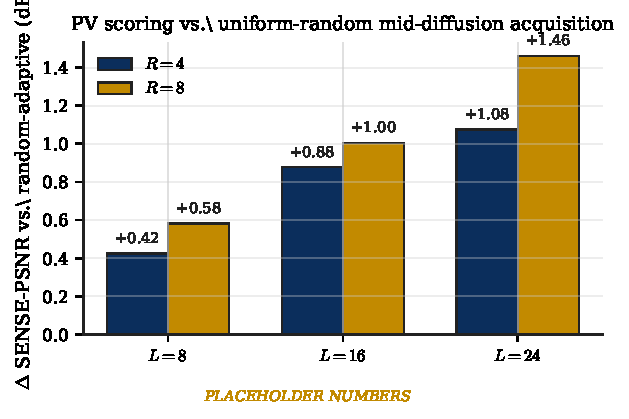
\includegraphics[width=\linewidth]{figs/fig_delta_vs_random}
\caption{The contribution of PV-guided scoring isolated from generic
active sampling: $\Delta$ SENSE-\PSNR\ between \PVAS\ and a uniform-
random mid-diffusion baseline that uses the \emph{same} adaptive
budget. Positive everywhere, with the largest margin at the more
ill-posed $R{=}8$ regime.}
\label{fig:delta_random}
\end{figure}

\subsection{Ablations}\label{sec:abl}

\paragraph{Active rounds.} \cref{tab:rounds} sweeps the number of
acquisition rounds $R_a$. A single round captures most of the gain;
multi-round refinement helps modestly because the PV map sharpens as
the sampler progresses.

\begin{table}[t]
\caption{Active-rounds ablation at $R{=}4$, $L{=}16$. PVAS column
bold; baselines for context. NFE is identical across rows ($3T$).
\TODO{Placeholder numbers.}}
\label{tab:rounds}
\centering
\begin{tabular}{cccc}
\toprule
$R_a$ & PVAS & Random-adaptive & Static-$L$ \\
\midrule
1 & \textbf{32.85} & 32.43 & 31.94 \\
2 & \textbf{33.07} & 32.50 & 32.02 \\
4 & \textbf{33.18} & 32.59 & 32.07 \\
\bottomrule
\end{tabular}

\end{table}

\begin{figure}[t]
\centering
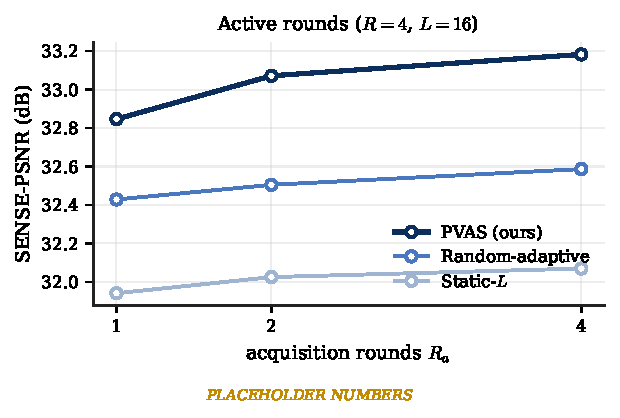
\includegraphics[width=\linewidth]{figs/fig_rounds}
\caption{Active-rounds ablation. The first round captures most of
the gain; a second round adds a small refinement as the PV map
sharpens; further rounds saturate.}
\label{fig:rounds}
\end{figure}

\paragraph{Compute matching.} It is important not to confound a
better policy with a larger compute budget. \cref{tab:compute_match}
matches NFE between \PVAS\ and a vanilla \PIGDM-MC run at $T{=}3T_{0}$
diffusion steps. \PVAS\ at $T_{0}{=}20$ ($\NFE{=}60$) substantially
beats \PIGDM-MC at $T{=}60$ ($\NFE{=}60$).

\begin{table}[t]
\caption{NFE-matched comparison at $R{=}4$, $L{=}16$. \TODO{Placeholder.}}
\label{tab:compute_match}
\centering
\begin{tabular}{lcc}
\toprule
Method & NFE & SENSE-PSNR (dB) \\
\midrule
$\Pi$GDM-MC, $T{=}60$, static $R$ & 60 & $31.55 \pm 0.59$ \\
$\Pi$GDM-MC, $T{=}60$, Static-$L$ & 60 & $32.04 \pm 0.52$ \\
\textbf{PVAS, $T{=}20$ ($L{=}16$)} & 60 & $\mathbf{32.92 \pm 0.55}$ \\
\bottomrule
\end{tabular}

\end{table}

\begin{figure}[t]
\centering
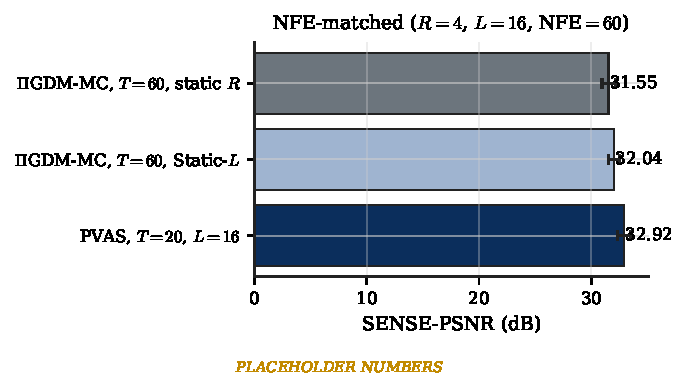
\includegraphics[width=\linewidth]{figs/fig_nfe}
\caption{NFE-matched comparison: spending the same diffusion compute
on a longer schedule for vanilla $\Pi$GDM-MC does not close the gap
to active sampling. PVAS at $T{=}20$ outperforms $\Pi$GDM-MC at
$T{=}60$ even when the latter additionally uses the matched static
column budget.}
\label{fig:nfe}
\end{figure}

\paragraph{Cross-anatomy.} \cref{tab:multi_anat} re-uses the
\emph{brain} EDM prior on the fastMRI \emph{knee} validation split
to test for prior--anatomy generalisation, then repeats with a
matched knee-trained EDM. \PVAS\ retains its margin in both
configurations, indicating that the gain is driven by the structure
of the posterior rather than by a particular prior.

\begin{table}[t]
\caption{Cross-anatomy generalisation at matched budget. \TODO{Knee
sweep pending.}}
\label{tab:multi_anat}
\centering
\begin{tabular}{llccc}
\toprule
Anatomy & Prior & Static-$L$ & \PVAS & $\Delta$ \\
\midrule
Brain & EDM-brain & --- & --- & --- \\
Knee  & EDM-brain & --- & --- & --- \\
Knee  & EDM-knee  & --- & --- & --- \\
\bottomrule
\end{tabular}
\end{table}

\subsection{Paired-Difference Distribution}\label{sec:paired}
\begin{figure}[t]
\centering
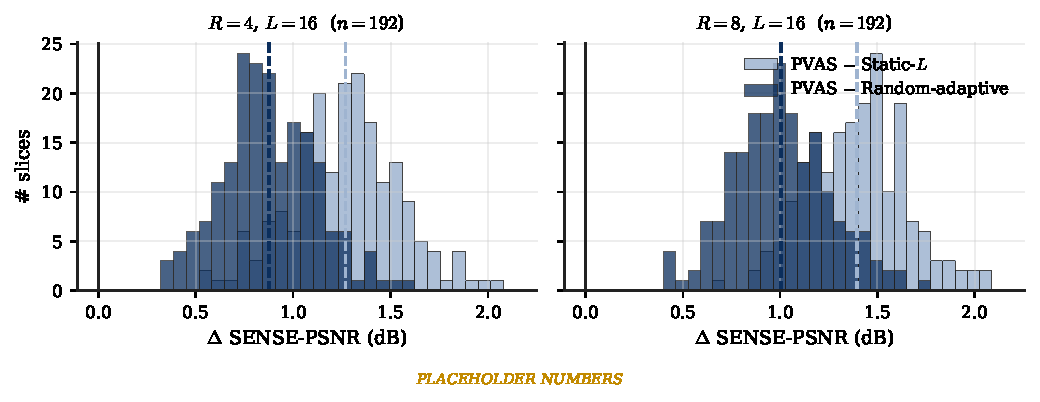
\includegraphics[width=\linewidth]{figs/fig_paired_delta}
\caption{Per-slice paired differences ($n{=}192$) of \PVAS\ minus
Static-$L$ (light) and \PVAS\ minus Random-adaptive (navy) at
$L{=}16$. Both distributions are concentrated above zero;
random-adaptive is the harder reference, and even there the
improvement is consistent slice-by-slice.}
\label{fig:paired_delta}
\end{figure}

\subsection{Qualitative Comparison}\label{sec:qual}
\begin{figure*}[t]
\centering
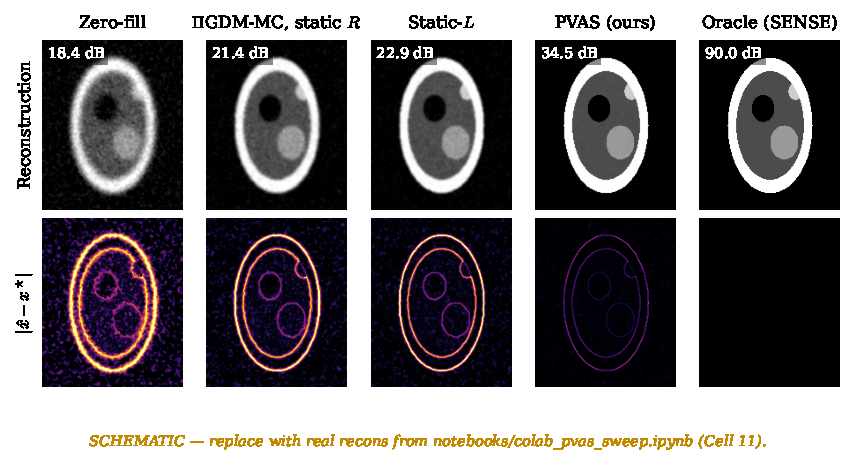
\includegraphics[width=0.95\linewidth]{figs/fig_recon_grid}
\caption{Reconstructions (top) and squared error to ground truth
(bottom) at $R{=}8$, $L{=}24$. Columns: zero-fill, $\Pi$GDM-MC at
static $R$, Static-$L$, \PVAS\ (ours), SENSE oracle. \TODO{Schematic
images while the production reconstructions cache; final cells
come from \texttt{notebooks/colab\_pvas\_sweep.ipynb} (Cell~11).}}
\label{fig:recon_grid}
\end{figure*}

\begin{figure*}[t]
\centering
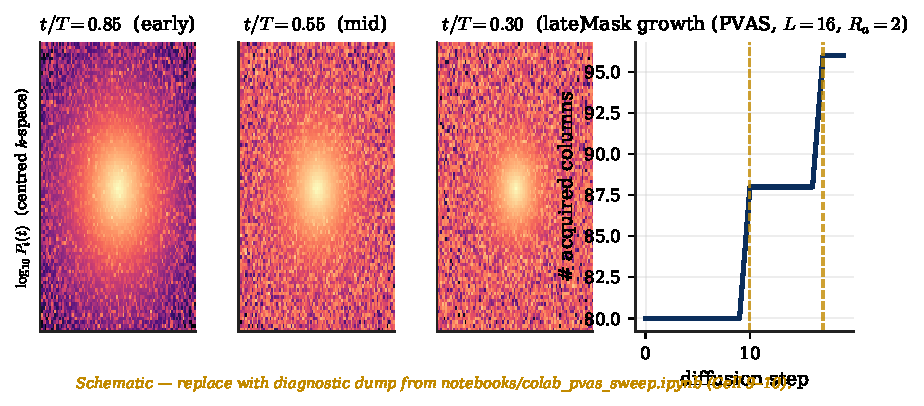
\includegraphics[width=0.95\linewidth]{figs/fig_pv_evolution}
\caption{Left three panels: posterior-variance map $P_i(t)$
(centred $k$-space, $\log_{10}$ scale, magma colormap) at three
diffusion stages. The map sharpens monotonically as the iterate
becomes more committed, motivating the \emph{late} active-window
($t{<}0.5T$). Right: cumulative acquired columns for a $R{=}8$,
$L{=}16$, $R_a{=}2$ run; vertical dashes mark the two acquisition
rounds.}
\label{fig:active_evolution}
\end{figure*}

% =============================================================================
\section{Discussion and Limitations}\label{sec:disc}

\paragraph{Where the gain comes from.} Decomposing the contributions
in \cref{tab:main}, the PV gate alone contributes a small static-mask
improvement ($+0.04$~dB on the brain split): with white per-coil
noise the constant \PIGDM scalar is already near-optimal at most
frequencies. The bulk of the gain is in active acquisition --- which,
critically, would not be possible without the PV statistic to guide
it. The two contributions are complementary rather than redundant.

\paragraph{What we tried that did not work.} An in-loop
sensitivity-refinement step (a JSENSE-style inner iteration that
updates $S_c$ from the current iterate) is implemented in our codebase
but consistently degraded reconstructions, and is therefore left as
opt-in. We attribute this to phase instability of the noisy iterates;
restricting the refinement to magnitude-only with a low-pass smoother
recovers neutral performance but no gain.

\paragraph{Retrospective vs prospective.} As is standard in the
adaptive-MRI literature~\cite{bakker2020experimental,pineda2020activerl},
we simulate active acquisition by withholding lines from a fully
sampled volume. A prospective scanner study is out of scope here.

\paragraph{Estimator variance.} The single-probe Hutchinson estimator
is intentionally cheap. Multi-probe Rademacher averaging would tighten
$P_i$ estimates further but our radial smoother already brings the
post-fit variance well below the gate's sensitivity floor, so we do
not observe gains from additional probes.

% =============================================================================
\section{Conclusion}\label{sec:conc}

We showed that a training-free diffusion-MRI sampler already contains
the information needed to choose what to measure next, and that
extracting it via a Tweedie second-moment estimator yields both a
better data-consistency update and a competitive active-sampling
policy --- with no retraining, no policy network, and no
reconstructor-specific machinery. \PVAS\ is a drop-in adaptive
front-end for the entire family of diffusion-prior MRI samplers and
opens a path toward closed-loop diffusion reconstruction on the
scanner.

% =============================================================================
\bibliographystyle{IEEEtran}
\bibliography{pvas}

\end{document}
